% Copyright 2004 by Till Tantau <tantau@users.sourceforge.net>.
%
% In principle, this file can be redistributed and/or modified under
% the terms of the GNU Public License, version 2.
%
% However, this file is supposed to be a template to be modified
% for your own needs. For this reason, if you use this file as a
% template and not specifically distribute it as part of a another
% package/program, I grant the extra permission to freely copy and
% modify this file as you see fit and even to delete this copyright
% notice. 

\documentclass[us]{beamer}
\usepackage[utf8]{inputenc}
\usepackage{babel}

% There are many different themes available for Beamer. A comprehensive
% list with examples is given here:
% http://deic.uab.es/~iblanes/beamer_gallery/index_by_theme.html
% You can uncomment the themes below if you would like to use a different
% one:
%\usetheme{AnnArbor}
%\usetheme{Antibes}
%\usetheme{Bergen}
%\usetheme{Berkeley}
%\usetheme{Berlin}
%\usetheme{Boadilla}
%\usetheme{boxes}
%\usetheme{CambridgeUS}
%\usetheme{Copenhagen}
%\usetheme{Darmstadt}
%\usetheme{default}
%\usetheme{Frankfurt}
%\usetheme{Goettingen}
%\usetheme{Hannover}
%\usetheme{Ilmenau}
%\usetheme{JuanLesPins}
%\usetheme{Luebeck}
\usetheme{Madrid}
%\usetheme{Malmoe}
%\usetheme{Marburg}
%\usetheme{Montpellier}
%\usetheme{PaloAlto}
%\usetheme{Pittsburgh}
%\usetheme{Rochester}
%\usetheme{Singapore}
%\usetheme{Szeged}
%\usetheme{Warsaw}

\title{Real Options Valuation: A Dynamic Programming Approach}

% A subtitle is optional and this may be deleted
%\subtitle{Optional Subtitle}

\author{Filip Rolenec}
% - Give the names in the same order as the appear in the paper.
% - Use the \inst{?} command only if the authors have different
%   affiliation.

\institute[CTU-FNSPE] % (optional, but mostly needed)
{
  \inst{}%
  Czech technical university in Prague\\
  FNSPE \\
  Department of Mathematics
 
}
% - Use the \inst command only if there are several affiliations.
% - Keep it simple, no one is interested in your street address.

\date{SPMS Conference, 20.09.2020}
% - Either use conference name or its abbreviation.
% - Not really informative to the audience, more for people (including
%   yourself) who are reading the slides online

\subject{Control Theory}
% This is only inserted into the PDF information catalog. Can be left
% out. 

% If you have a file called "university-logo-filename.xxx", where xxx
% is a graphic format that can be processed by latex or pdflatex,
% resp., then you can add a logo as follows:

% \pgfdeclareimage[height=0.5cm]{university-logo}{university-logo-filename}
% \logo{\pgfuseimage{university-logo}}

% Delete this, if you do not want the table of contents to pop up at
% the beginning of each subsection:
%\AtBeginSubsection[]
%{
%  \begin{frame}<beamer>{Outline}
%    \tableofcontents[currentsection,currentsubsection]
%  \end{frame}
%}

% Let's get started
\begin{document}

\begin{frame}
  \titlepage
\end{frame}

\begin{frame}{Table of contents}
  \tableofcontents
  % You might wish to add the option [pausesections]
\end{frame}

% Section and subsections will appear in the presentation overview
% and table of contents.

\section{Introduction}

\subsection{General}

\begin{frame}{Introduction}{General}

	\begin{columns}
		\column{0.5\textwidth}
 		\begin{itemize}
 			\item {Financial options}
			\item {Real option analysis (ROA)}
			\item {Stochastic decision theory (SDT)}
		\end{itemize}	
		\column{0.5\textwidth}
		\begin{figure}
			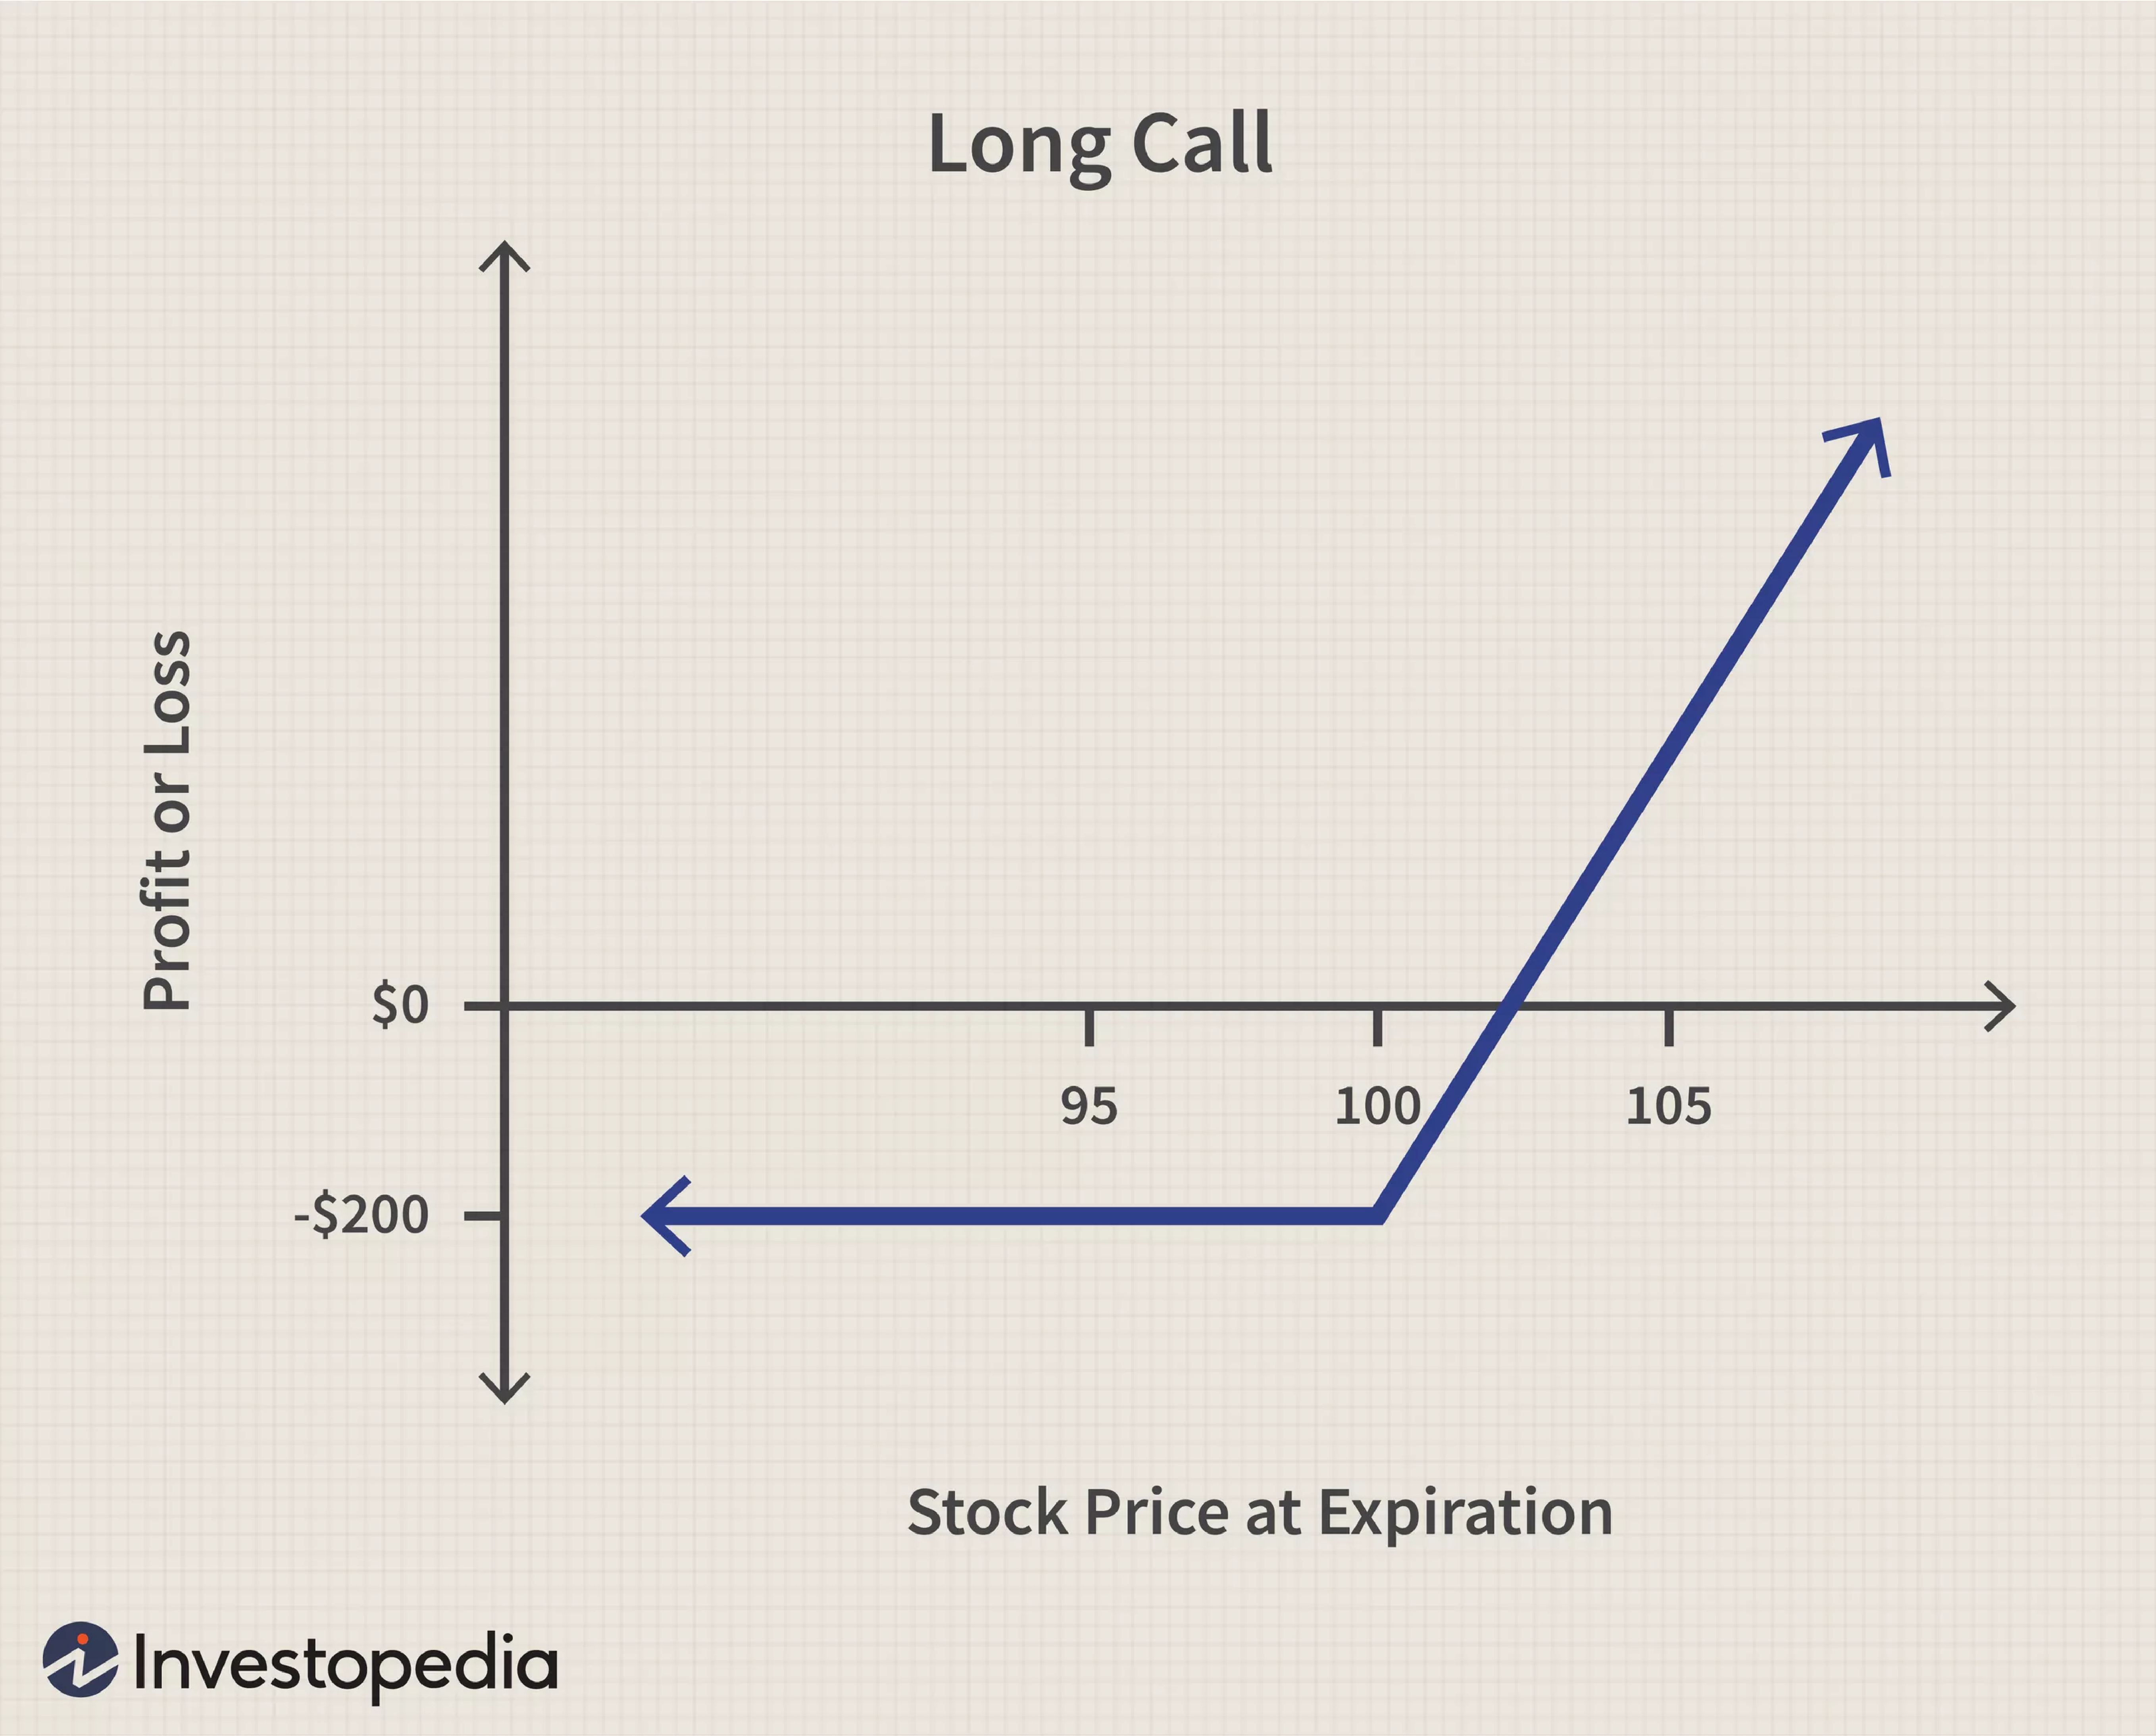
\includegraphics[scale=0.06]{Long_call.pdf}
			\caption{Call Option \cite{Investopedia}}
		\end{figure}
\end{columns}	

\end{frame}

\subsection{Detailed}

\begin{frame}{Introduction}{Detailed}

\begin{columns}
	\column{0.5\textwidth}
	\begin{itemize}
		\item {Three classes of ROA authors (BSM model analogy)}
		\item {SDT framework $>$ frameworks used in economy}
		\item {Formulation of ROA problem in SDT framework}
	\end{itemize}	
	\column{0.5\textwidth}
	\begin{figure}
		\includegraphics[scale=0.35]{Guthrie.png}
		\caption{Economical framework example \cite{Guthrie}}
	\end{figure}
\end{columns}	

\end{frame}




\section{ROA interpreted in SDT}

\subsection{ROA inspiration - Guthrie}

\begin{frame}{ROA inspiration}{Graeme Guthrie}
  \begin{itemize}
  	\begin{columns}
  		\column{0.50\textwidth}
  		
  \item { Replicating portfolio (efficient markets) }
  \item { Risk neutral probabilities }
  \item { Backward induction }
  
  \item{Probability of up and down move \cite{Guthrie}: }
  
  \begin{equation}
  	\pi_u=\frac{ZR_f-X_d}{X_u-X_d}, \pi_d=\frac{X_u -ZR_f}{X_u-X_d}
  \end{equation}
  
  \column{0.40\textwidth}
  \begin{figure}
 \includegraphics[scale=0.3]{risk_neutral.png}
 \caption{Binomial model}
  \end{figure}
  
\end{columns}
  \end{itemize}
\end{frame}

\subsection{ROA - limitations}

\begin{frame}{ROA limitations}{General}
	\begin{itemize}
		\item {Limited number of uncertainty sources - one (efficient market)}
		\item {Simple distributions - binomial model}
		\item {Limited by computational complexity for higher-dimensional problems}
		\item {Complicated scaling in types and scale of real options}
	\end{itemize}
\end{frame}

\subsection{SDT - Improvements}

\begin{frame}{SDT Improvements}{General}
	\begin{itemize}
		\item {Allows for multiple sources of uncertainty - seamless integration}
		\item {Allows continuous distributions, theoretically of any type}
		\item {Computational complexity tools - ADP}
		\item {Real options (actions) easily scaled with action set}
	\end{itemize}

	Furthermore: 
	\begin{itemize}
		\item{Allows for simple integration of Bayesian learning}
		\item{Allows for complex creation of prior probability densities}
	\end{itemize}
\end{frame}

\begin{frame}{SDT Improvements}{Preserving economical truths}
	\begin{itemize}
		\item {Time value of money - discounting factors}
		\item {Risk aversion of investors - utility theory }
		\item {Risk-neutral probabilities - Bayesian priors}
	\end{itemize}
\end{frame}


\begin{frame}{SDT Improvements}{ADP}
		\begin{itemize}
			\item{To be done}
		\end{itemize}
\end{frame}

\section{Experiments}

\subsection{Gas power plant}
	
	
	\begin{frame}{Valuation of gas power plant}{General Idea}
	\begin{itemize}
		\item {Power generating company}
		\item {In the next 5 years, possibility to build 200MW or 400MW gas unit for 65/130M EUR}
		\item {Prices of gas, power, CO2 allowances are 24EUR, 9EUR, 40EUR per MWh}
		\item {Government policy favoring renewables can rise -> higher volatility of prices.}
		\item {Lifespan of gas power plant is set to 25 years, loan possible with 3\% interest rate}
		\item {Power plant is selling its power as monthly contracts}		
	\end{itemize}
	\end{frame}

	\begin{frame}{Valuation of gas power plant}{Details}
	Considered real options:
	\begin{itemize}
		\item {Wait for more favorable market prices - Timing option }
		\item {Build 200MW gas power plant. Then possibility to increase to 400MW - Scaling option}
		\item {Sell the power plant - abandonment option}
		\item {Mothball the plant. It is not able to produce, but the fixed costs are lowered} 
		\item {Ability to not run the power plant (paying fixed costs)- switching option}
	\end{itemize}
	
	Sources of uncertainty: 
	\begin{itemize}
		\item {Price of gas, power and CO2 - lognormal process with different volatilities}
		\item {Government policy for renewables  - discrete with positive mean}
	\end{itemize}	
	\end{frame}
	

	\begin{frame}{Results}
	\begin{itemize}
		\item {To be computed}
	\end{itemize}
	\end{frame}


\section*{Summary}

\begin{frame}{Summary}
	Contributions: 
  	\begin{itemize}
  	\item {Item}
  	\item {Item} 
  	\item {Item}
  	\item {Item}
  	\end{itemize}
  
  \begin{itemize}
  \item{Possible directions of future research:}
    \begin{itemize}
    \item{Item}
    \item{Item}
    \item{Item}
    \end{itemize}
  \end{itemize}
\end{frame}



% All of the following is optional and typically not needed. 
\appendix
\section<presentation>*{\appendixname}
\subsection<presentation>*{Reference}

\begin{frame}[allowframebreaks]
  \frametitle<presentation>{Reference}
   
  \begin{thebibliography}{10}
     \bibitem{Agent} Thebftonline.com. (2018). The process of corporate decision making – ( 5) | Business \& Financial Times Online. [online] Available at: https://thebftonline.com/features/the-process-of-corporate-decision-making-5/ [Accessed 3 Apr. 2018].
    \bibitem{Coin} Istockphoto.com. (2018). Royalty Free Coin Flip Pictures, Images and Stock Photos - iStock. [online] Available at: https://www.istockphoto.com/photos/coin-flip [Accessed 3 Apr. 2018].
  \bibitem{Peterka}
  Mys.utia.cas.cz. (2018). BAYESIAN APPROACH TO SYSTEM IDENTIFICATION. [online] Available at: http://mys.utia.cas.cz:1800/educalibre/checkout/pracovni/examples2010/theory/peterka.pdf [Accessed 2 Apr. 2018].
 

  \bibitem{Putterman} M. L. Markov decision processes: discrete stochastic dynamic programming. (John Wiley \& Sons, 1994).
   
  \bibitem{Bellman} Bellman, R. Dynamic programming. (Princenton University Press, 1957).
   
  \end{thebibliography}
\end{frame}

\end{document}


